\documentclass[aspectratio=169,11pt]{beamer}

\usetheme{Madrid}
\usecolortheme{default}
\usepackage[T1]{fontenc}
\usepackage[utf8]{inputenc}
\usepackage{graphicx}
\usepackage{booktabs}
\usepackage{tikz}
\usepackage{array}
\usetikzlibrary{arrows.meta,positioning,shapes.geometric,fit}

\definecolor{siteblue}{RGB}{0,113,188}
\definecolor{sitegreen}{RGB}{30,145,95}
\definecolor{siteorange}{RGB}{230,126,34}
\definecolor{sitedark}{RGB}{34,40,49}
\definecolor{sitelight}{RGB}{246,247,241}

\setbeamercolor{structure}{fg=siteblue}
\setbeamercolor{frametitle}{fg=white,bg=sitedark}
\setbeamercolor{title}{fg=white,bg=sitedark}
\setbeamercolor{block title}{fg=white,bg=siteblue}
\setbeamercolor{block body}{fg=sitedark,bg=blue!3}
\setbeamertemplate{navigation symbols}{}
\setbeamertemplate{footline}[frame number]
\setlength{\parskip}{0.2em}

\newcommand{\hkulogo}{%
  \begin{tikzpicture}[baseline=-0.45ex]
    \node[
      draw=gray!45,
      line width=0.35pt,
      fill=white,
      rounded corners=1.2pt,
      inner xsep=2.2pt,
      inner ysep=1.2pt
    ] {
\includegraphics[width=2.35cm]{figures/hku_logo.png}};
  \end{tikzpicture}%
}

\setbeamertemplate{background}{%
  \begin{tikzpicture}[remember picture,overlay]
    \node[anchor=north east,xshift=-0.28cm,yshift=-0.06cm] at (current page.north east) {\hkulogo};
  \end{tikzpicture}%
}
\addtobeamertemplate{frametitle}{}{%
  \begin{tikzpicture}[remember picture,overlay]
    \node[anchor=north east,xshift=-0.28cm,yshift=-0.16cm] at (current page.north east) {\hkulogo};
  \end{tikzpicture}%
}

\title[Construction Robot Digital Twin]{Construction Robot Digital Twin}
\subtitle{Autonomous Navigation to a Wall-Mounted AprilTag}
\author{TAN TIAN\\CIVIL 8025 Project 4}
\institute{ROS2 + Gazebo + Nav2 + Local Web Dashboard}
\date{April 30, 2026}

\newcommand{\topic}[1]{\textcolor{siteblue}{\textbf{#1}}}
\newcommand{\githubbadge}{%
  \href{https://github.com/skywalker0525/8025_pj4}{%
    \raisebox{-0.12cm}{
\includegraphics[height=0.42cm]{figures/github_logo.png}}%
    \hspace{0.35em}%
    {\scriptsize\texttt{github.com/skywalker0525/8025\_pj4}}%
  }%
}

\begin{document}

\begin{frame}
  \titlepage
  \begin{tikzpicture}[remember picture,overlay]
    \node[anchor=north east,xshift=-0.28cm,yshift=-0.06cm] at (current page.north east) {\hkulogo};
  \end{tikzpicture}
  \vspace{-0.8em}
  \begin{center}
    \small Four-wheel inspection robot, physics-based simulation, SLAM-ready map workflow, and browser-based operator interface.

    \vspace{0.75em}
    \githubbadge
  \end{center}
\end{frame}

\begin{frame}{Presentation Roadmap}
  \begin{columns}[T,onlytextwidth]
    \begin{column}{0.48\textwidth}
      \begin{block}{What I built}
        \begin{itemize}
          \item A ROS2 construction robot digital twin
          \item Gazebo world with collision constraints
          \item Nav2 mission from start point A to AprilTag target
        \end{itemize}
      \end{block}
    \end{column}
    \begin{column}{0.48\textwidth}
      \begin{block}{What I will show}
        \begin{itemize}
          \item Robot model and control interfaces
          \item Navigation, SLAM, telemetry, and safety
          \item Final video demo after the slides
        \end{itemize}
      \end{block}
    \end{column}
  \end{columns}
\end{frame}

\begin{frame}{Project Goal}
  \small
  \begin{block}{Background}
    Construction sites are dynamic, cluttered, and safety-critical. Autonomous mobile robots can support inspection by navigating site-like areas, checking target locations, and giving operators live feedback.
  \end{block}

  \begin{block}{Inspection task}
    The robot starts at point \topic{A}, autonomously navigates through a construction-like indoor environment, approaches a wall-mounted \topic{AprilTag}, and reports the mission as complete.
  \end{block}

  \vspace{-0.25em}
  \begin{columns}[T,onlytextwidth]
    \begin{column}{0.57\textwidth}
      \begin{itemize}
        \item Mobile robot must obey physical and collision constraints.
        \item Operator can switch between automatic mission and manual control.
        \item Dashboard gives live feedback instead of relying only on RViz.
      \end{itemize}
    \end{column}
    \begin{column}{0.38\textwidth}
      \begin{block}{Task pipeline}
        \begin{enumerate}
          \item Start from A.
          \item Plan with Nav2.
          \item Approach AprilTag.
          \item Report \texttt{DONE}.
        \end{enumerate}
      \end{block}
    \end{column}
  \end{columns}
\end{frame}

\begin{frame}{Digital Twin Architecture}
  \centering
  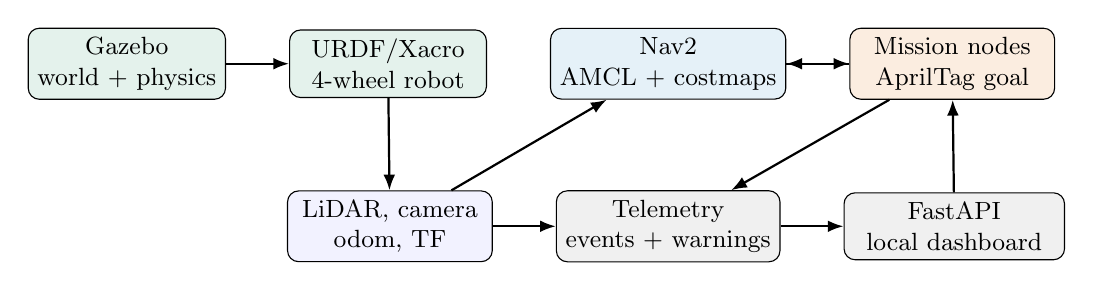
\begin{tikzpicture}[
    node distance=0.6cm and 0.8cm,
    box/.style={draw,rounded corners,align=center,minimum height=0.85cm,font=\small},
    arrow/.style={-{Latex[length=2mm]},thick}
  ]
    \node[box,fill=sitegreen!12,minimum width=2.4cm] (world) {Gazebo\\world + physics};
    \node[box,fill=sitegreen!12,right=of world,minimum width=2.5cm] (robot) {URDF/Xacro\\4-wheel robot};
    \node[box,fill=siteblue!10,right=of robot,minimum width=2.4cm] (nav2) {Nav2\\AMCL + costmaps};
    \node[box,fill=siteorange!14,right=of nav2,minimum width=2.6cm] (mission) {Mission nodes\\AprilTag goal};
    \node[box,fill=gray!12,below=1.15cm of nav2,minimum width=2.8cm] (telemetry) {Telemetry\\events + warnings};
    \node[box,fill=gray!12,right=of telemetry,minimum width=2.8cm] (web) {FastAPI\\local dashboard};
    \node[box,fill=blue!5,left=of telemetry,minimum width=2.6cm] (sensors) {LiDAR, camera\\odom, TF};

    \draw[arrow] (world) -- (robot);
    \draw[arrow] (robot) -- (sensors);
    \draw[arrow] (sensors) -- (nav2);
    \draw[arrow] (nav2) -- (mission);
    \draw[arrow] (mission) -- (nav2);
    \draw[arrow] (mission) -- (telemetry);
    \draw[arrow] (sensors) -- (telemetry);
    \draw[arrow] (telemetry) -- (web);
    \draw[arrow] (web) -- (mission);
  \end{tikzpicture}

  \vspace{0.8em}
  \small The dashboard is an experience layer over ROS topics, actions, and services; it does not replace Gazebo or RViz engineering tools.
\end{frame}

\begin{frame}{Robot and Environment Model}
  \begin{columns}[T,onlytextwidth]
    \begin{column}{0.48\textwidth}
      \begin{block}{Robot}
        \begin{itemize}
          \item Four-wheel differential/skid-steer base
          \item Rear left/right wheels driven by one Gazebo diff-drive plugin
          \item Passive front wheels for stable contact
          \item Pan/tilt camera gimbal with joint limits
          \item LiDAR, RGB camera, odometry, and TF
        \end{itemize}
      \end{block}
    \end{column}
    \begin{column}{0.48\textwidth}
      \begin{block}{Construction scene}
        \begin{itemize}
          \item Walls and floor with collision bodies
          \item Barriers, material stacks, tool chest, rebar cage
          \item Simple cylinder column for stable obstacle geometry
          \item Wall-mounted AprilTag target
          \item Static map plus SLAM workflow
        \end{itemize}
      \end{block}
    \end{column}
  \end{columns}
\end{frame}

\begin{frame}{Autonomous Mission}
  \begin{columns}[T,onlytextwidth]
    \begin{column}{0.55\textwidth}
      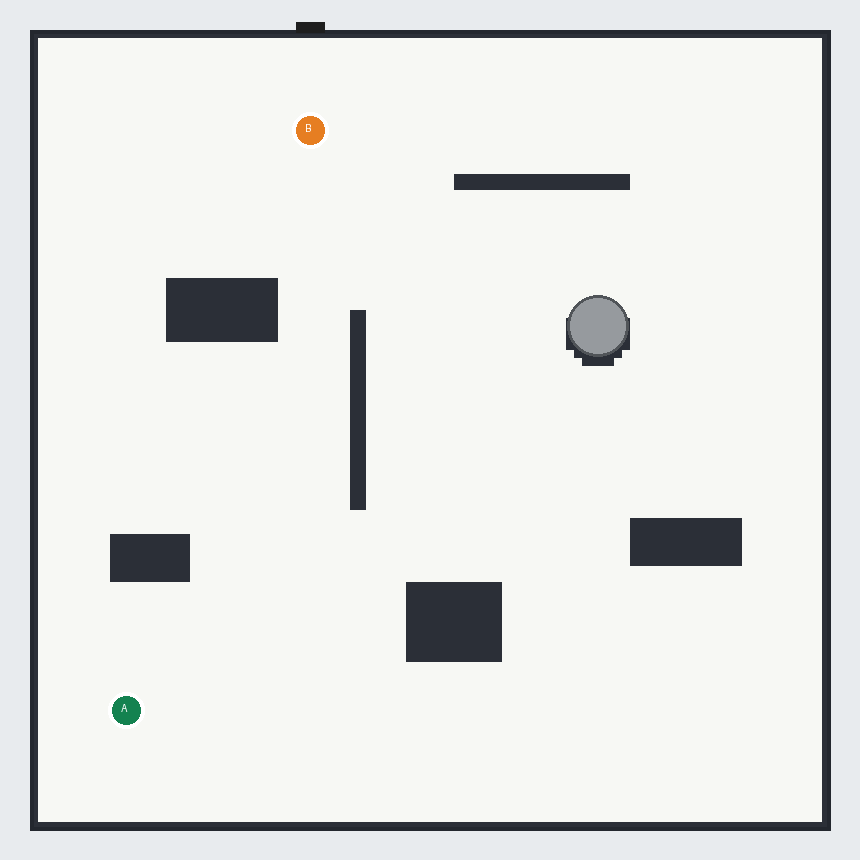
\includegraphics[width=\linewidth]{figures/route_map.png}
    \end{column}
    \begin{column}{0.42\textwidth}
      \small
      \begin{block}{Mission sequence}
        \begin{enumerate}
          \item Publish AMCL initial pose at A
          \item Wait for \texttt{NAV2\_READY}
          \item Send B as \texttt{NavigateToPose}
          \item Approach the AprilTag wall
          \item Publish \texttt{APRILTAG\_REACHED}
        \end{enumerate}
      \end{block}
      \vspace{0.5em}
      \begin{block}{Map information}
        \begin{itemize}
          \item Static map: \texttt{room\_map.yaml}
          \item Resolution: $0.1\,m/cell$
          \item Size: $100 \times 100$ cells
          \item Coverage: about $10\,m \times 10\,m$
        \end{itemize}
      \end{block}
    \end{column}
  \end{columns}
\end{frame}

\begin{frame}{Web Dashboard}
  \begin{columns}[T,onlytextwidth]
    \begin{column}{0.54\textwidth}
      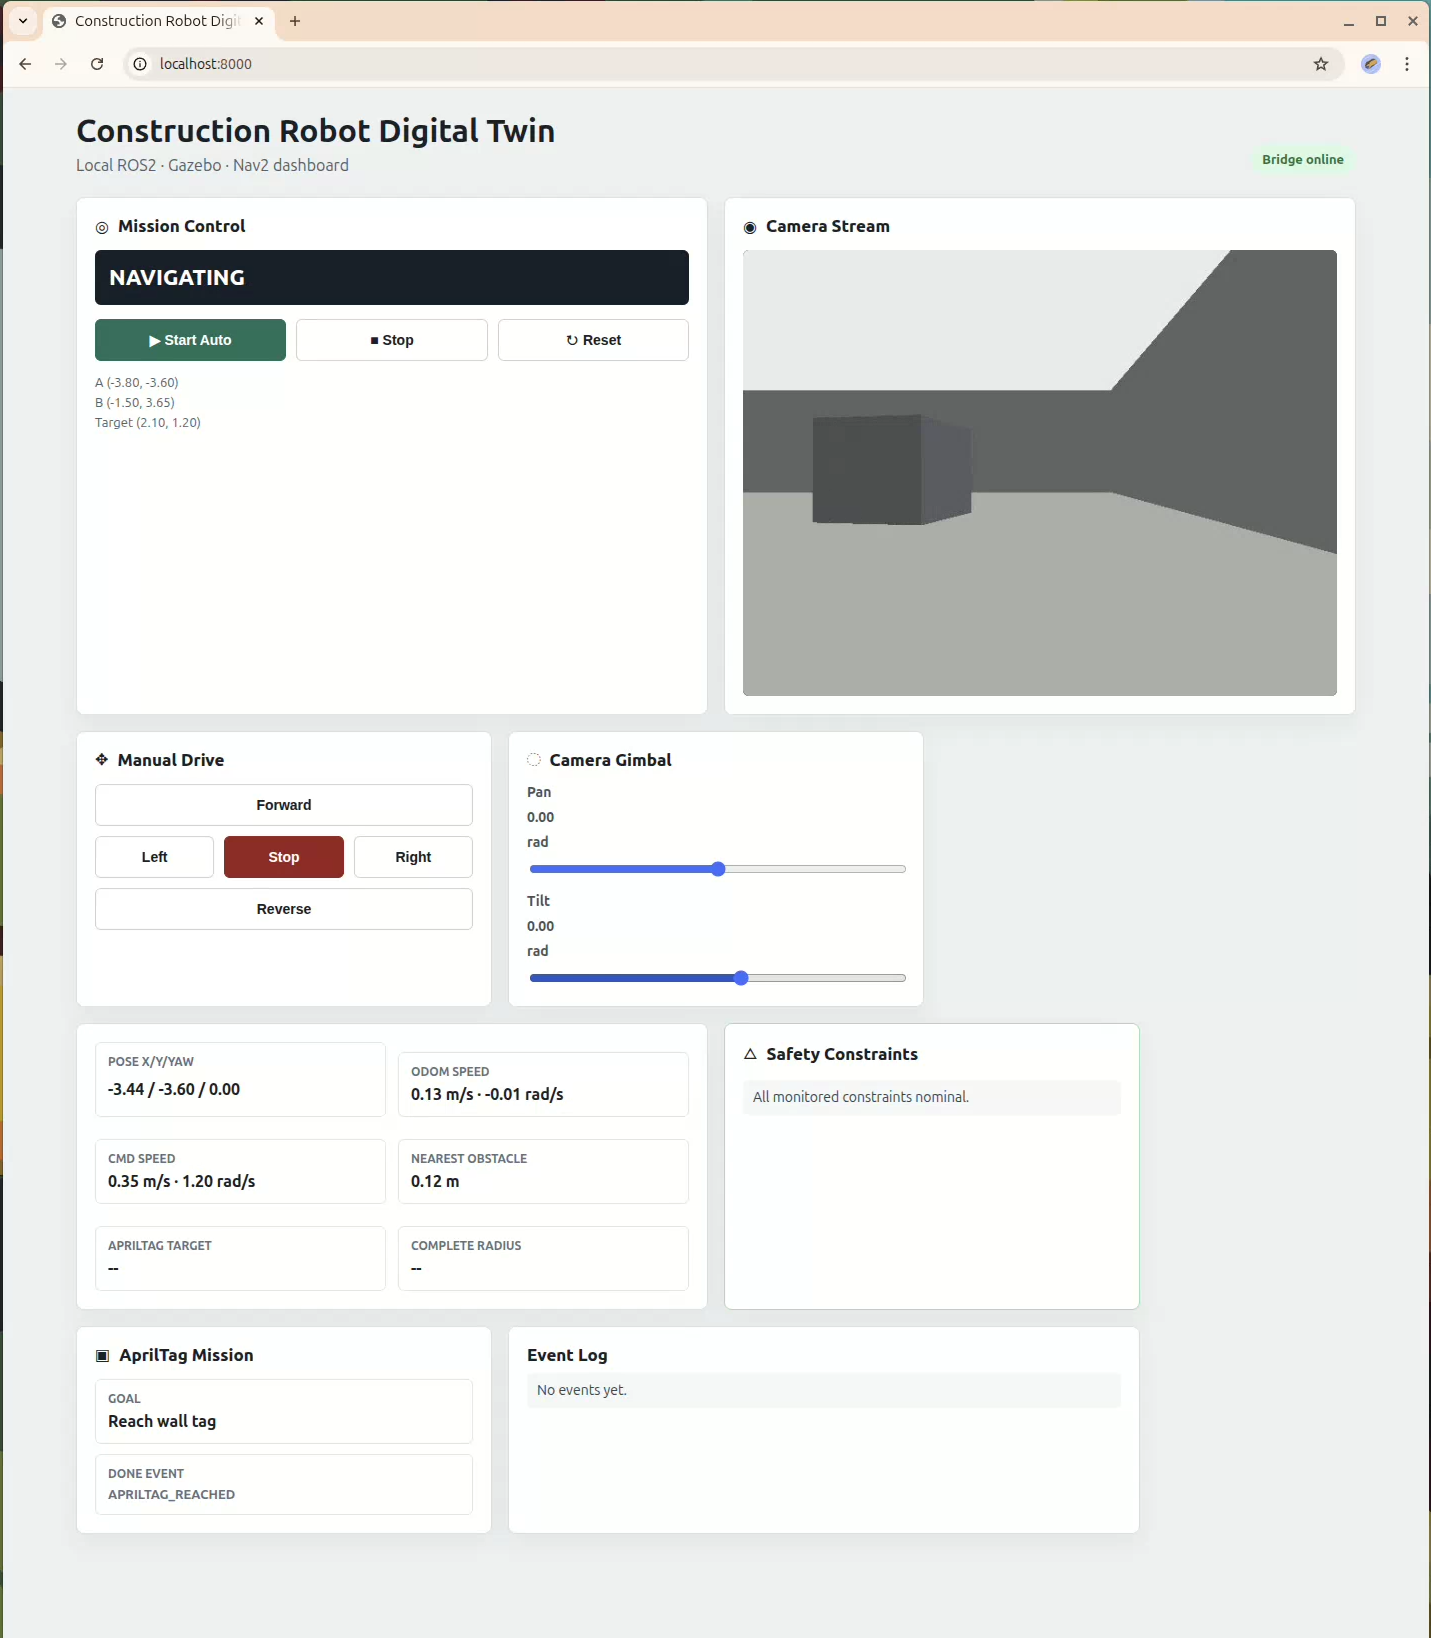
\includegraphics[height=0.78\textheight]{figures/web.png}
    \end{column}
    \begin{column}{0.43\textwidth}
      \begin{block}{Operator controls}
        \begin{itemize}
          \item Start Auto, Stop, Reset
          \item Manual forward, reverse, left, right
          \item Camera pan and tilt sliders
          \item Local camera stream endpoint
        \end{itemize}
      \end{block}
      \begin{block}{Live feedback}
        \begin{itemize}
          \item Mission state and event log
          \item Pose, velocity, command velocity
          \item Nearest LiDAR obstacle range
          \item AprilTag target information
          \item Safety warning panel
        \end{itemize}
      \end{block}
    \end{column}
  \end{columns}
\end{frame}

\begin{frame}{SLAM and Map Workflow}
  \begin{columns}[T,onlytextwidth]
    \begin{column}{0.52\textwidth}
      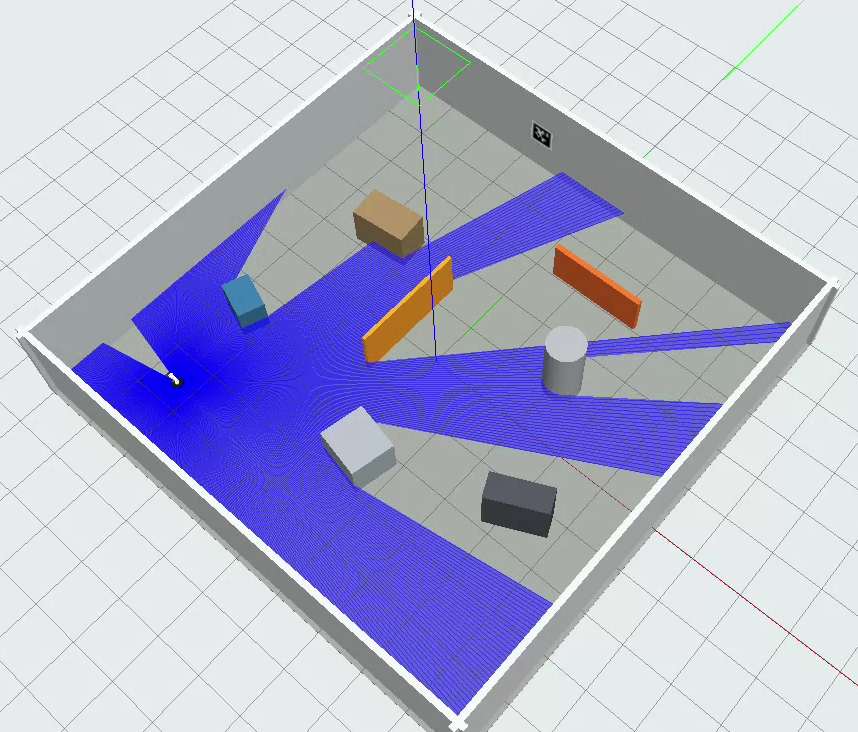
\includegraphics[width=\linewidth,height=0.69\textheight,keepaspectratio]{figures/map.png}
    \end{column}
    \begin{column}{0.45\textwidth}
      \scriptsize
      \begin{block}{Mapping mode}
        \begin{itemize}
          \setlength\itemsep{0.15em}
          \item Launch Gazebo with SLAM Toolbox
          \item Drive manually from the dashboard
          \item RViz shows the LiDAR-built \texttt{/map}
          \item Save the map for Nav2
        \end{itemize}
      \end{block}
      \vspace{-0.25em}
      \begin{block}{Navigation mode}
        \begin{itemize}
          \setlength\itemsep{0.15em}
          \item Load \texttt{room\_map.yaml}
          \item AMCL estimates \texttt{map -> odom}
          \item Diff-drive publishes \texttt{odom -> base\_link}
          \item Nav2 plans through costmaps
        \end{itemize}
      \end{block}
    \end{column}
  \end{columns}
\end{frame}

\begin{frame}{Safety and Physical Constraints}
  \begin{columns}[T,onlytextwidth]
    \begin{column}{0.49\textwidth}
      \begin{block}{Model-level constraints}
        \begin{itemize}
          \item URDF collision geometry and inertia
          \item Wheel contact and friction parameters
          \item Gimbal pan/tilt joint limits
          \item Gazebo collision for walls and obstacles
        \end{itemize}
      \end{block}
    \end{column}
    \begin{column}{0.49\textwidth}
      \begin{block}{Runtime constraints}
        \begin{itemize}
          \item Nav2 obstacle and inflation layers
          \item Maximum linear and angular speeds
          \item Nearest obstacle distance warning
          \item Emergency \texttt{STOP} publishes zero velocity
        \end{itemize}
      \end{block}
    \end{column}
  \end{columns}

  \vspace{0.7em}
  \begin{center}
    \large Safety evidence is visible in code, costmaps, telemetry, and the dashboard.
  \end{center}
\end{frame}

\begin{frame}{Implementation Highlights}
  \begin{columns}[T,onlytextwidth]
    \begin{column}{0.32\textwidth}
      \begin{block}{Simulation}
        \small
        \texttt{my\_robot\_sim}\\
        Gazebo world, wall AprilTag, obstacles, robot spawn.
      \end{block}
    \end{column}
    \begin{column}{0.32\textwidth}
      \begin{block}{Navigation}
        \small
        \texttt{my\_robot\_navigation}\\
        Nav2 parameters, map, waypoints, RViz, SLAM launch.
      \end{block}
    \end{column}
    \begin{column}{0.32\textwidth}
      \begin{block}{Mission + Web}
        \small
        \texttt{my\_robot\_mission}\\
        Readiness checks, events, telemetry, manual control, markers.
      \end{block}
    \end{column}
  \end{columns}

  \vspace{0.9em}
  \begin{itemize}
    \item \texttt{START\_AUTO} waits for Nav2 action server and \texttt{map -> base\_link}.
    \item The mission reports failures explicitly using \texttt{NAV2\_NOT\_READY} events.
    \item The system can be run reproducibly with Docker and tmux.
  \end{itemize}
\end{frame}

\begin{frame}{Limitations and Future Work}
  \begin{columns}[T,onlytextwidth]
    \begin{column}{0.48\textwidth}
      \begin{block}{Current limitations}
        \begin{itemize}
          \item AprilTag is currently a visual target and known map goal.
          \item Dashboard shows telemetry, but RViz remains stronger for detailed costmap inspection.
          \item Real-world deployment would need calibration and sensor noise handling.
        \end{itemize}
      \end{block}
    \end{column}
    \begin{column}{0.48\textwidth}
      \begin{block}{Next steps}
        \begin{itemize}
          \item Add real AprilTag image detection overlay.
          \item Stream LiDAR/costmap view directly into the dashboard.
          \item Use tag pose estimation for final visual servoing.
        \end{itemize}
      \end{block}
    \end{column}
  \end{columns}
\end{frame}

\begin{frame}{Conclusion}
  \begin{block}{What the project demonstrates}
    \begin{itemize}
      \item A complete construction robot digital twin with physics, sensors, navigation, and operator interface.
      \item Autonomous navigation from A to a wall-mounted AprilTag target.
      \item Evidence of collision modelling, costmap-based planning, telemetry, and safety constraints.
      \item A reproducible Docker/tmux workflow for demonstration and future development.
    \end{itemize}
  \end{block}

  \vspace{0.8em}
  \begin{center}
    \Large Next: \href{pj4.webm}{recorded mission video}.
  \end{center}
\end{frame}

\end{document}
